In this chapter, we deal with the perspective camera approach to Shape
from Shading problems. This approach differs from the Orthographic
Approach and can be considered to be a much more realistic approach to
shape from shading. In orthographic projection, we assume that the
light direction is given by a single vector $\mathbf{L} = (\alpha,
\beta, \gamma)$ and that the light rays are parallel to the retinal
plane. In perspective projection model, however the light rays are not
assumed to be parallel in case of perspective projection. This enables
us to reduce the number of singular points in the image. See Figure
(\ref{fig:2})
\begin{figure}[h!]
  \centering
  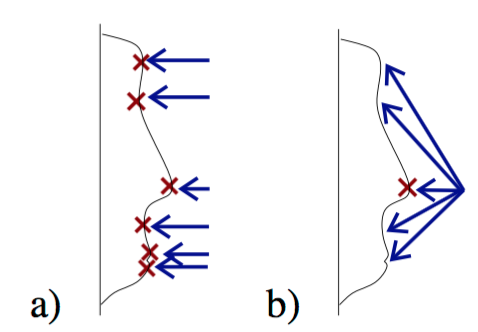
\includegraphics[scale = 0.5]{images/ovsp.png}
  \caption{a) Orthographic vs b) Perspective :
    Number of Singular Points}
  \label{fig:2}
\end{figure}

\noindent
In the perspective projection, the camera can be assumed to be placed at
the \textbf{focal point}, or at \textbf{infinity}. Prados and
Faugeras\cite{prados1} obtained a generic Hamiltonian for a perspective camera
approach  that unifies these conditions. However, the approach still
had the problem of singular points and the information at these points
must be specified apriori at these points to single out the unique
solution. So, Prados et.al\cite{prados2} came up with a modified brightness
equation to remove the notion of singular points. In this chapter, we
discuss the derivation of the HJE that describes the model, and
address existence and uniqueness of a viscosity solution.

\section{Mathematical Model}
In this section, we derive the Hamilton Jacobi Equation for
perspective model, using the modified brightness equation\cite{prados2}. Let
$\Omega \subset \mathbb{R}^2$. Let the scene be described by a
surface $\mathbb{S}$, which is parametrized by a function $S : \Omega
\to \mathbb{R}^3$,
\begin{equation}
  \mathbb{S} = \{S(x), \;\; x \in \bar{\Omega}\}
\end{equation}
Now, let us assume that the light source is placed on the focal
point. Figure (\ref{fig:3a}) represents the current setup in a
perspective projection model.\\
\begin{figure}
  \begin{subfigure}{0.5\textwidth}
    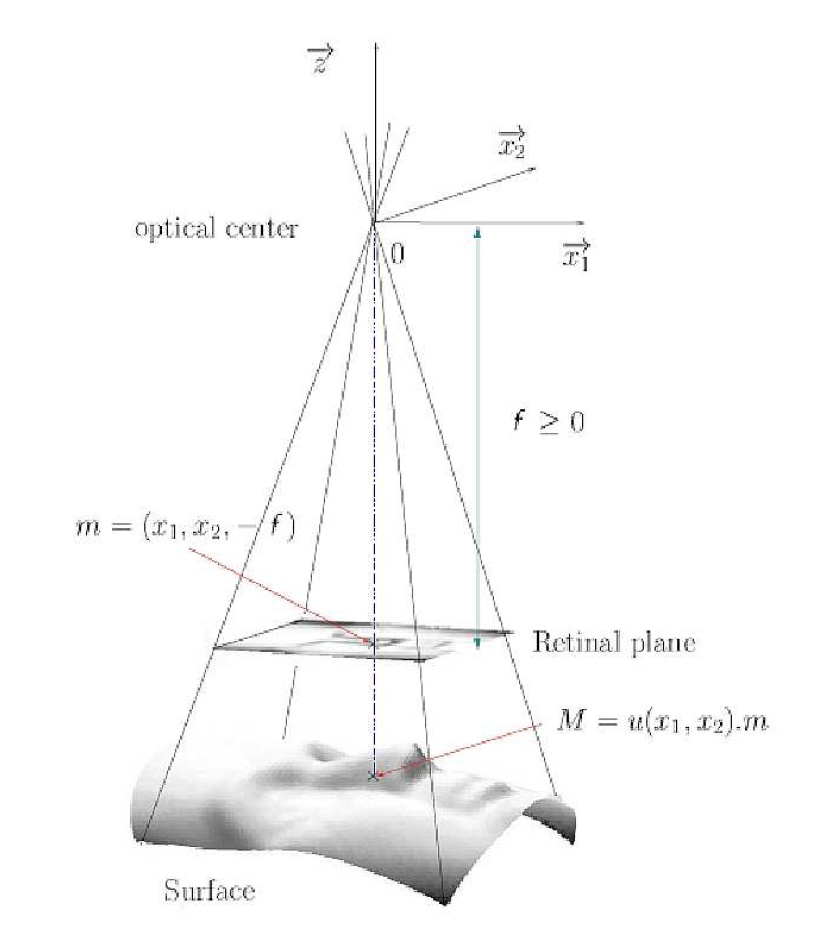
\includegraphics[scale = 0.5]{images/persp2.png}
    \subcaption{The scene}
    \label{fig:3a}
  \end{subfigure}
  \begin{subfigure}{0.5\textwidth}
    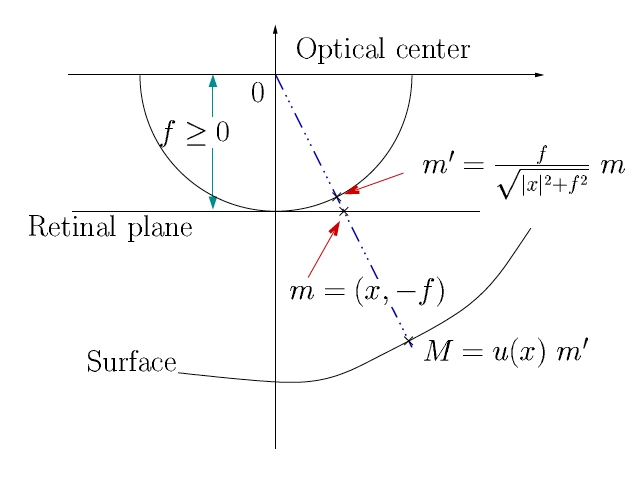
\includegraphics[scale = 0.65]{images/persp1.png}
    \subcaption{Surface representation}
    \label{fig:3b}
  \end{subfigure}
  \caption{Perspective Projection Model}
\end{figure}

\noindent
From Figure (\ref{fig:3b}), we can deduce that the parametrization of
the surface is given by,
\begin{equation}
  S(x) = \frac{fu(x)}{\sqrt{\lvert x \rvert^2 + f^2}} (x,-f)
\end{equation}

\noindent
where $f$ is the focal length of the camera. To simplify the model, Prados et.al in their previous work\cite{prados1}, used the
brightness equation
\begin{equation}
  R(x) = \cos \theta \label{eq:15}
\end{equation}
where $\theta$ is the angle between the Light Vector and the surface
unit normal and $R(x)$ is the irradiance of the surface. This gave a HJE which
suffered from singular points. So to overcome this difficulty, Prados
et.al\cite{prados2} did not neglect the $\frac{1}{r^2}$ attenuation term in their
model, which would normally be neglected to simplify the
model. Contrary to this statement, adding the attenuation term would
make the model better posed.\\

\noindent
The image irradinace equation (\ref{eq:15}), now becomes,
\begin{equation}
  R(x) = \frac{\cos \theta}{r^2}\label{eq:16}
\end{equation}
where $r = fu(x)$ is the distance between the light source and the considered
surface point $u(x)$. Assuming that the surface is lambertian and the camera is placed at the focal point, we have the unit light vector $L$ and the
surface unit normal $n$,
\begin{eqnarray}
  L(S(\mathbf{x})) &=& \frac{1}{\sqrt{\lvert \mathbf{x} \rvert^2+f^2}} (\mathbf{x},-f)\label{eq:17}\\
  n(\mathbf{x}) &=& \left( f\nabla u(\mathbf{x}) -
  \frac{fu(\mathbf{x})}{\lvert \mathbf{x} \rvert^2 + f^2} \mathbf{x},\;\;
  \nabla u(\mathbf{x}).\mathbf{x} + \frac{f u(\mathbf{x})}{\lvert
  \mathbf{x} \rvert^2 + f^2} f\right)\label{eq:18}
\end{eqnarray}

\noindent
Using (\ref{eq:16}) - (\ref{eq:18}), and $I(\mathbf{x}) = \cos \theta = L(\mathbf{x}).n(\mathbf{x})$, we
obtain the equation,
\begin{equation}
  I(\mathbf{x})f^2 \frac{\sqrt{f^2|\nabla u(\mathbf{x})|^2 + (\nabla
      u(\mathbf{x}).\mathbf{x})^2/Q(\mathbf{x})^2 +
      u(\mathbf{x})^2}}{u(\mathbf{x})} - u(\mathbf{x})^{-2} = 0
\end{equation}

\noindent
Assuming that the surface is visible, that is $u(\mathbf{x}) > 0$, we
make a change of variables $v = \ln u$. This gives us the HJE,
\begin{equation}
  -e^{-2v} + \frac{I(\mathbf{x})f^2}{Q(\mathbf{x})} \sqrt{f^2 |\nabla
    v(\mathbf{x})|^2 + (\nabla v(\mathbf{x}). \mathbf{x})^2 +
    Q(\mathbf{x})^2} = 0 \label{eq:19}
\end{equation}
where $Q(\mathbf{x}) = \sqrt{\frac{f^2}{|\mathbf{x}|^2 +
    f^2}}$. (\ref{eq:19}) is the HJE that describes the
setting. Solving for $u(\mathbf{x})$ with the known parameters $f,I$
gives the reconstructed 3D object. In the next section, we briefly
discuss the existence and uniqueness of the solution to (\ref{eq:19}).

\section{Existence and Uniqueness}
Consider the following Dirichlet boundary value problem,
\begin{eqnarray}
  -e^{-2v} + \frac{I(x)f^2}{Q(x)} \sqrt{f^2|\nabla u|^2 + (x.\nabla
    u)^2 + Q(x)^2} = 0 \qquad \text{in} \;\;\; \Omega \label{eq:20}\\
  u(x) = \varphi(x) \qquad \text{on} \;\;\; \partial \Omega \label{eq:21}
\end{eqnarray}

\noindent
Let us denote the Hamiltonian of the problem by $H(x,v,p)$, $p =
\nabla v$. The following two theorems gives the condition for the
existence and uniqueness of solution to the Prados model.
\begin{theorem}
  \textbf{Existence of continuous viscosity solution to the Prados
    Model}\\
  If
  \begin{itemize}
  \item
    (A1) \textbf{Regularity} : $H \in C^0(\bar{\Omega} \times \mathbb{R}^n)$
  \item
    (A2) \textbf{Convexity} : $H$ is convex with respect to $\mathbf{p} \;\;\forall
    \;\;\mathbf{x} \in \bar{\Omega}$
  \item
    (A3) \textbf{Subsolution} : $\inf_{\mathbf{p} \in \mathbb{R}^2}
    H(\mathbf{x},u,\mathbf{p}) \le 0 $ in $\bar{\Omega}$
  \item
    (A4) \textbf{Uniform Coercivity} : $H(\mathbf{x},u,\mathbf{p}) \to +\infty$
    when $|\mathbf{p}| \to \infty$ uniformly with respect to $x \in
    \bar{\Omega}$.
  \item
    (A5) $u(\mathbf{x}) = \varphi(\mathbf{x})$ satisfies the compatibity condition.
  \end{itemize}
  then $u$ is a continuous viscosity solution of the Hamilton Jacobi Equation.
\end{theorem}

\begin{theorem}
  \textbf{Uniqueness of solution to the Prados
    Model}\\
  If
  \begin{itemize}
  \item
    (A1) \textbf{Convexity} : $H$ is convex with respect to $\mathbf{p} \;\;\forall
    \;\;\mathbf{x} \in \bar{\Omega}$
  \item
    (A2) \textbf{Space variable regularity} : There exists a modulus $m$ such
    that $\forall \mathbf{x},\mathbf{y} \in \bar{\Omega}$ and
    $\mathbf{p}\in\mathbb{R}^2$, $|H(\mathbf{x},u,\mathbf{p}) -
    H(\mathbf{y},u,\mathbf{p})| \le m(|x-y|(1+|p|))$
  \item
    (A3) \textbf{Strict Subsolution} : There exists a strict viscosity
    subsolution $\underset{\bar{}}{u}$, such that
    $H(\mathbf{x},\underset{\bar{}}{u}, \mathbf{p}) < 0 \;\; \forall
    \;\; \mathbf{x}\in\Omega$
  \end{itemize}
  then there exists atmost one continuous viscosity solution to the
  HJE such that $u(\mathbf{x}) = \varphi(\mathbf{x})$ on the boundary.
\end{theorem}

\noindent
A rigorous proof for existence and uniquness can be found
in \cite{prados2}. Most of the conditions like convexity and regularity of the
Hamiltonian can be easily verified. The most interesting property in
the theorem is the subsolution condition. The Hamiltonian $H(x,u,p)$
satisfies the subsolution condition, if
\begin{eqnarray}
  &\implies&\inf_{p\in\mathbb{R}^2}H(x,u,p) \le 0 \\
  &\implies& -e^{-2u} + I(x)f^2 \le 0 \quad \forall \;\; x \in \Omega\\
  &\implies& I(x)f^2 \le e^{-2v} \\
  &\implies& v \le -\frac{1}{2} \ln (I(x)f^2) \label{eq:22}
\end{eqnarray}

\noindent
(\ref{eq:22}) can be reformulated as
\begin{equation}
  \implies v_0 = -\frac{1}{2}\ln(\min_{x\in\Omega} I(x)f^2) \label{eq:23}
\end{equation}

\noindent
(\ref{eq:22}) assures that a unique viscosity solution exists to the
problem. (\ref{eq:23}) can be supplied as an initial condition to evolution
type schemes to ensure convergence of the numerical scheme to the
exact solution. The notion of singular points disappear in this case as
long as (\ref{eq:22}) is satisfied. This is not assured in other cases\cite{prados1,prad,prad2}
because of the absence of the $e^{-2u}$ term in the Hamiltonian and
thus the subsolution condition is violated at these points. Thus, this
model has a unique viscosity solution that satisfies the HJE in
$\Omega$ and $\varphi(x)$ on $\partial \Omega$.\\

\noindent
In the next chapter, we discuss the numerical schemes used to solve
Hamilton Jacobi Equations.
